\section{Pianificazione}
\textit{TechSweave} ha deciso di pianificare il progetto in base alle scadenze sotto riportate. Di conseguenza il progetto è stato suddiviso nelle seguenti fasi:
\begin {itemize}
\item Analisi;
\item Consolidamento dei Requisiti;
\item Progettazione architetturale;
\item Progettazioni di dettaglio e codifica;
\item Validazione e collaudo;
\end {itemize}
Ognuna di queste fasi verrà suddivisa in attività da realizzare entro i tempi stabiliti per la fase stessa e sarà mostrata nei rispettivi diagrammi di Gantt\textsubscript{\textbf{G}}.
\subsection{Analisi}
\textit{Periodo: dal 2021-03-11 al 2021-04-02}
Questo periodo corrisponde alla data di formazione del gruppo e termina con la data ultima per la consegna dei documenti relativi alla \textit{Revisione dei Requisiti}.\\
Questa fase è stata scomposta nelle seguenti attività che corrispondono ai documenti prodotti:
\begin {itemize}
\item \textbf{Studio di Fattibilità:} viene effettuato uno studio dei capitolati comprendente i lati positivi e negativi a essi collegati, per poi selezionarne uno. L'attività è bloccante per l'\textit{Analisi dei Requisiti};
\item \textbf{Norme di Progetto:} vengono specificate tutte le regole da rispettare durante lo sviluppo del progetto. Da questo documento dipenderanno le norme di stesura di tutti i prodotti successivi;
\item \textbf{Analisi dei Requisiti:} vengono studiati ed analizzati i requisiti legati al capitolato scelto nello \textit{Studio di Fattibilità};
\item \textbf{Piano di Progetto:} il presente documento in cui attività, compiti e risorse precedentemente analizzate vengono distribuite tra i membri del team. Nel seguente documento è presente il calcolo del preventivo per la realizzazione del progetto;
\item \textbf{Piano di Qualifica:} vengono individuati i metodi necessari per garantire la qualità del prodotto;
\item \textbf{Glossario:} documento contenente tutti i termini che possono risultare ambigui durante lo svolgimento del progetto, di essi viene fornita una definizione sintetica ma esaustiva.
\end {itemize}
\begin{figure}[!ht]
    \caption{Diagramma di Gantt della fase di Analisi}
    \vspace{5px}
    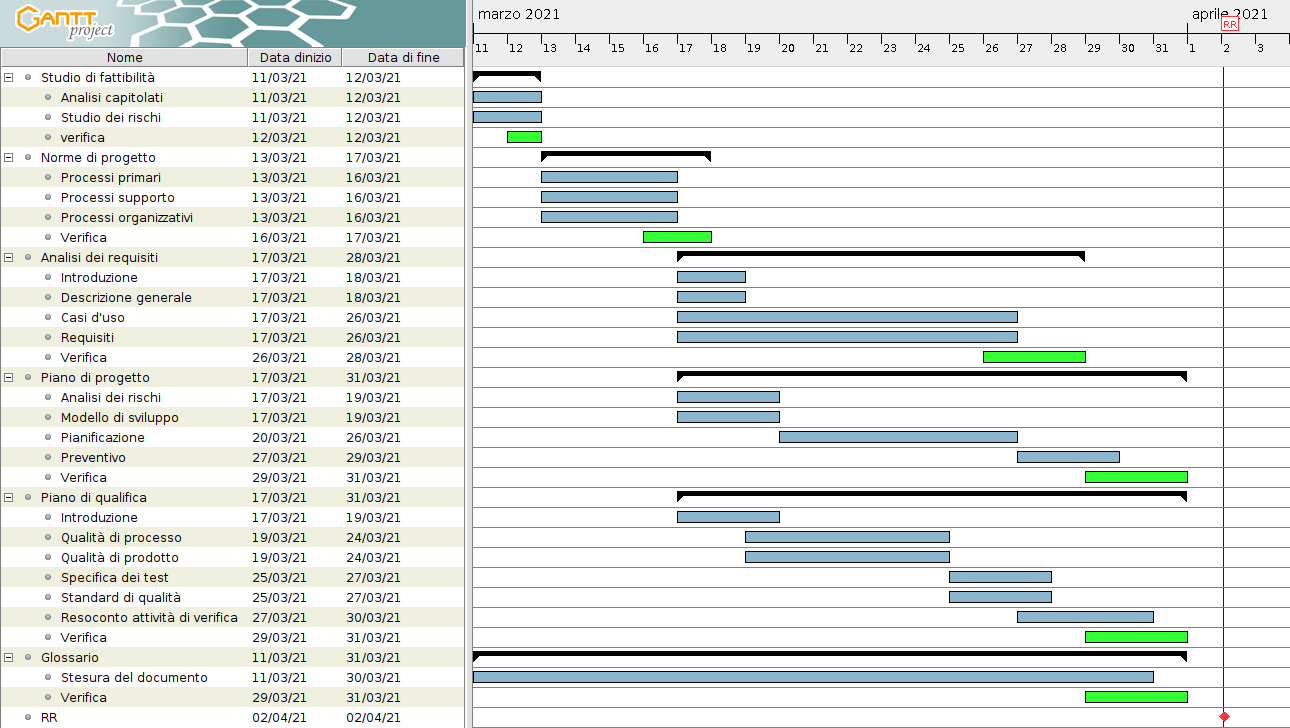
\includegraphics[scale=0.21]{../../../Images/Diagrammi/Gantt/diagramma_gantt_analisi_0.2.png}
    \centering
\end{figure}

\subsection{Consolidamento dei requisiti}
\textit{Periodo: dal 2021-04-02 al 2021-04-09}\\
Questa fase comincia con la fine di quella di Analisi e termina il giorno della presentazione della \textit{Revisione dei Requisiti}. Le attività di questa fase sono:
\begin {itemize}
\item \textbf{Consolidamento:} con lo scopo di consolidare e migliorare i requisiti ottenuti nella fase precedente;
\item \textbf{Preparazione alla presentazione:} per preparare il materiale necessario alla presentazione del 2021-04-09;
\item \textbf{Incremento e Verifica:} nella quale vengono migliorati i documenti prodotti nella fase precedente se necessario;
\item \textbf{Approfondimento personale:} ogni componente del gruppo dovrà dedicare delle ore di studio autonomo e approfondimento riguardo alle tecnologie necessarie per sviluppare il prodotto.
\end {itemize}
\begin{figure}[!ht]
    \caption{Diagramma di Gantt della fase di consolidamento dei requisiti}
    \vspace{5px}
    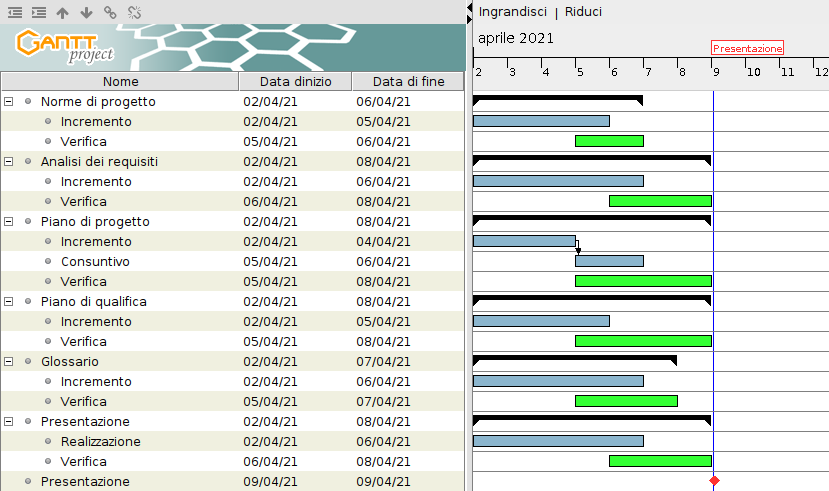
\includegraphics[scale=0.4]{../../../Images/Diagrammi/Gantt/consolidamento.png}
    \centering
\end{figure}

\subsection{Progettazione architetturale}
\textit{Periodo: dal 2021-04-09 al 2021-05-03}\\
Questa fase comincia il giorno successivo alla presentazione e la sua fine coincide con la data di consegna della \textit{Revisione di Progettazione}. In questo lasso di tempo verrà individuata una soluzione architetturale che soddisfi i requisiti richiesti.\\
Le attività di questa fase sono:
\begin {itemize}
\item \textbf{Incremento e verifica:} in cui i documenti precedentemente redatti vengono aggiornati e migliorati;
\item \textbf{Technology Baseline\textsubscript{\textbf{G}}:} viene fatta un’analisi ad alto livello per comprendere appieno le tecnologie coinvolte, scegliendo l’architettura del codice e i design pattern\textsubscript{\textbf{G}} che saranno adoperati per lo sviluppo. Viene codificato il Proof of Concept\textsubscript{\textbf{G}} che sarà presentato o condiviso tramite repository con committente e proponente per verificare il corretto sviluppo del software.
\end {itemize}
\begin{figure}[!ht]
    \caption{Diagramma di Gantt dell’attività di progettazione architetturale}
    \vspace{5px}
    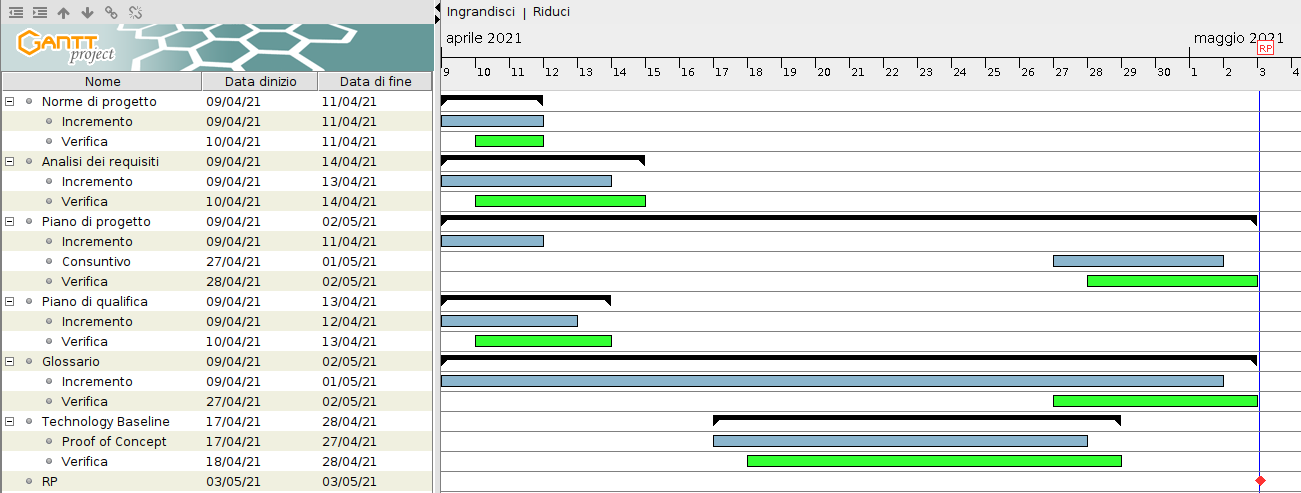
\includegraphics[scale=0.3]{../../../Images/Diagrammi/Gantt/progettArchitetturale_v2.png}
    \centering
\end{figure}

\subsection{Progettazione di dettaglio e codifica}
\textit{Periodo: dal 2021-05-10 al 2021-06-04}\\
L’inizio di questa fase è il giorno della scadenza della \textit{Revisione di Progettazione} e la data di fine coincide con la data di consegna dei documenti in vista della \textit{Revisione di Qualifica}.\\
Le attività di questa fase sono:
\begin {itemize}
\item \textbf{Incremento e verifica:} in cui i documenti precedentemente redatti vengono aggiornati e migliorati;
\item \textbf{Product Baseline\textsubscript{\textbf{G}}}: a seguito della \textit{Technology Baseline} l’architettura individuata in essa viene scomposta nelle sue unità, che vengono analizzate in profondità per fornire i dettagli necessari alla loro codifica e verifica;
\item \textbf{Codifica:} questa attività consiste nella scrittura e verifica del codice secondo i modi definiti nel \textit{Piano di Qualifica}.
\item \textbf{Specifica Tecnica:} Viene redatto un documento contenente tutte le caratteristiche del prodotto e le motivazioni che hanno portato alla loro scelta;
\item \textbf{Manuale Utente:} viene redatto un documento contenente le istruzioni d'uso del software da parte dell'utente.
\end {itemize}
\begin{figure}[!ht]
    \caption{Diagramma di Gantt dell’attività di progettazione di dettaglio e codifica}
    \vspace{5px}
    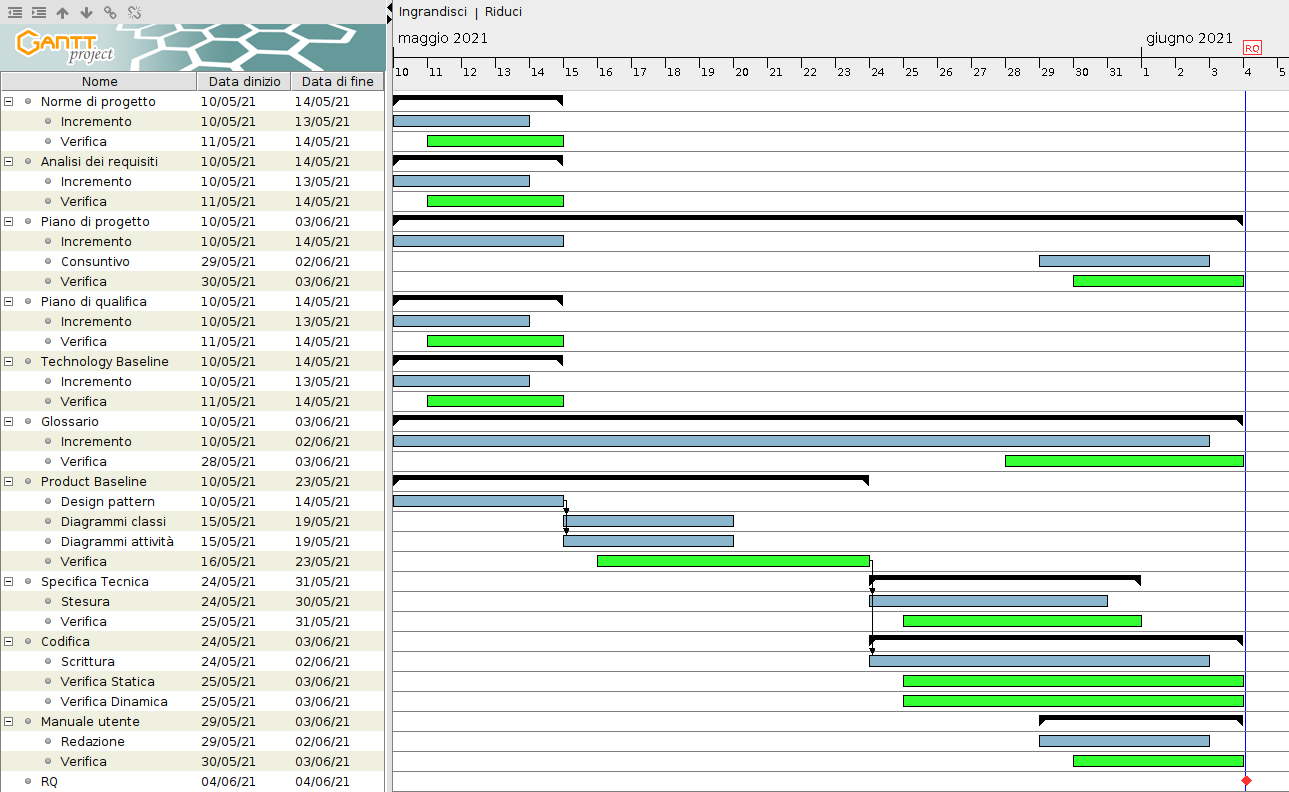
\includegraphics[scale=0.22]{../../../Images/Diagrammi/Gantt/progettazioneCodifica_v2.png}
    \centering
\end{figure}

\subsection{Validazione e collaudo}
\textit{Periodo: dal 2021-06-11 al 2021-07-02}\\
L’inizio di questa fase è il giorno della scadenza della \textit{Revisione di Qualifica} e la data di fine coincide con la data di consegna dei documenti in vista della \textit{Revisione di Accettazione}.\\
Le attività di questa fase sono:
\begin {itemize}
\item \textbf{Incremento e verifica:} in cui i documenti precedentemente redatti vengono aggiornati e migliorati;
\item \textbf{Validazione e collaudo:} per la parte di collaudo si eseguiranno ulteriori test sul prodotto, in modo da garantirne correttezza e stabilità. Per ciò che concerne la validazione, verrà valutata la coerenza del prodotto e dei requisiti specificati nel documento \textit{Analisi dei Requisiti} nella sua ultima versione;
\end {itemize}
\begin{figure}[!ht]
    \caption{Diagramma di Gantt dell’attività di Validazione e Collaudo}
    \vspace{5px}
    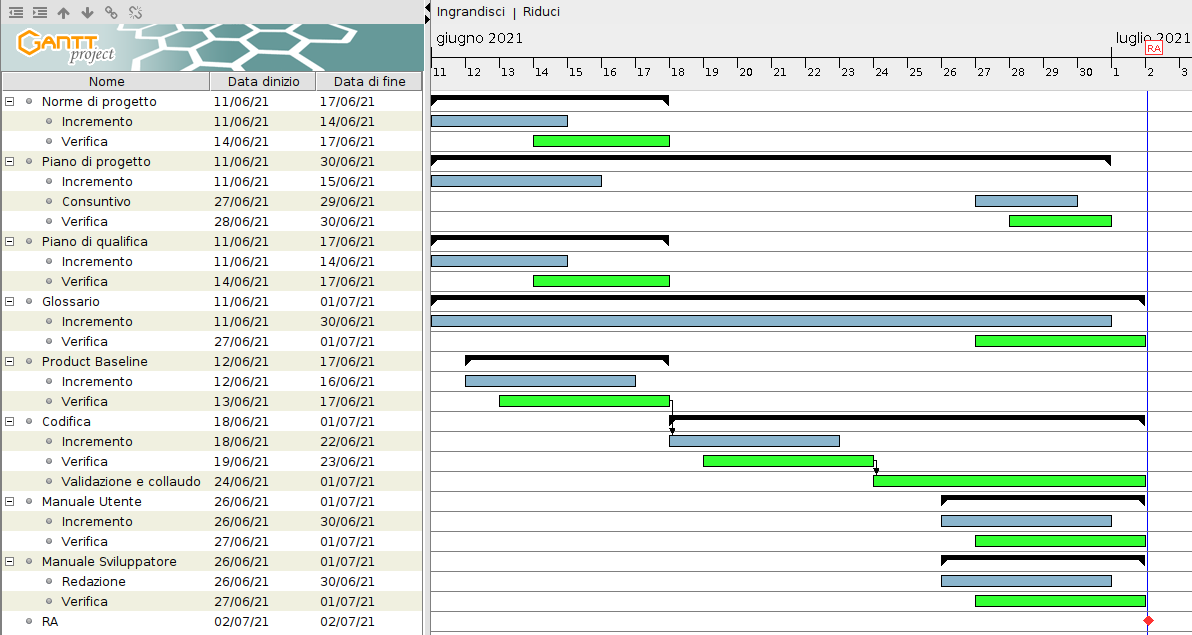
\includegraphics[scale=0.3]{../../../Images/Diagrammi/Gantt/validazione_v2.png}
    \centering
\end{figure}